\documentclass[12pt, titlepage, twoside]{amsart}

\usepackage[a4paper, margin=1in]{geometry}
\usepackage{amsmath}
\usepackage[foot]{amsaddr}
\usepackage{enumitem}
\usepackage[dvipsnames]{xcolor}
\usepackage{parskip}
\usepackage{esvect}
\usepackage{minted}
\usepackage{hyperref}
\usepackage{graphicx}

\newcommand{\R}{\ensuremath{\mathbb R}}
\newcommand{\Z}{\ensuremath{\mathbb Z}}
\newcommand{\N}{\ensuremath{\mathbb N}}

\setminted{linenos, breaklines}
\hypersetup{
  colorlinks=true,
  linkcolor=Orchid,
  urlcolor=ProcessBlue
}


\graphicspath{ {.} }

\raggedright

\begin{document}

\title[ScottyRank.jl]{ScottyRank.jl: An Implementation of PageRank \& HITS}

\author{Siyuan Chen}
\author{Michael Zhou}
\email{siyuanc2@andrew.cmu.edu}
\email{mhzhou@andrew.cmu.edu}
\date{November 2021}

\begin{abstract}
  SOME ABSTRACT HERE
\end{abstract}

\maketitle

\tableofcontents

\section{Mathematical Background}

\subsection{Linear Algebra}

\subsubsection{Definitions}

Positive matrices are defined as matrices with positive entries.

Markov matrices are defined as square matrices with nonnegatives entries and column sum $1$ across all of its columns.
Note that for a $n\times n$ matrix $M$, the latter condition is equivalent to $M^T\vec{1} = \vec{1}$,
where $\vec{1}\in\R^n$ has all ones as components.

Positive Markov matrices are defined as, well, positive Markov matrices.

\subsubsection{Facts}

(Perron-Frobenius theorem)
Let $A$ be a positive square matrix.
Let $\lambda_1$ be $A$'s maximum eigenvalue in terms of absolute values.
Then $\lambda_1$ is positive and has algebraic (and subsequently geometric) multiplicity $1$.

Let $M$ be a Markov matrix.
Let $\lambda_1$ be $M$'s maximum eigenvalue in terms of absolute values.
Then $\lambda_1 = 1$.

Let $M'$ be a positive Markov matrix.
Let $\lambda_1$ be $M'$'s maximum eigenvalue in terms of absolute values.
Then $\lambda_1 = 1$ and has algebraic (and subsequently geometric) multiplicity $1$.

\subsubsection{Usage}

Let $M$ be a $n\times n$ Markov matrix.
Then $M$ specifies a dicrete memoryless transition process between $n$ states, namely the process where
\[
  \left(\forall (t, i, j)\in\N\times[n]\times[n]\right)
  \left[\Pr(\text{state }i\text{ at time }t + 1\mid \text{state }j\text{ at time }t) = M_{ij}\right].
\]

Let $\vec{v}\in\R^n$ such that $\vec{v}$ has nonnegative components and $\vec{v}^T\vec{1} = 1$ (a stochastic vector).
Then $\vec{v}$ specifies an (initial) discrete probability distribution over the $n$ states, namely the distribution where
\[
  (\forall i\in[n])
  [\Pr(\text{state }i\text{ at time }0) = \vec{v}_i].
\]

Then the probability distribution over the $n$ states after $t$ steps of the transition process specified by $M$ is precisely $M^t\vec{v}$,
or equivalently
\[
  (\forall (t, i)\in\N\times[n])
  \left[\Pr(\text{state }i\text{ at time }t) = \left(M^t\vec{v}\right)_i\right].
\]

\subsection{Graph Theory}

\subsubsection{Definitions}

A simple directed graph is defined as an unweighted directed graph without self-referential edges or multiple edges
between the same origin destination pair.

For a simple directed graph with $n$ vertices, the adjacency matrix $\mathcal{A}$ is defined to be
the $n\times n$ matrix where
\[
  (\forall (i, j)\in[n]\times[n])\left(A_{ij} = 
    \begin{cases}
      1 & \text{there is an edge to $i$ from $j$} \\
      0 & \text{otherwise}
    \end{cases}
  \right).
\]

\subsubsection{Facts}

For a simple directed graph with $n$ vertices and its adjacency matrix $\mathcal{A}$,
\begin{align*}
  (\forall j\in[n])&
  \left[\text{number of outgoing neighbors from vertex $j$} = \mathrm{out}(j) = (\mathcal{A}_{*j})^T\vec{1}\right] \\
  (\forall i\in[n])&
  \left[\text{number of incoming neighbors to vertex $i$} = \mathrm{in}(i) = (\mathcal{A}_{i*})^T\vec{1}\right].
\end{align*}

\section{Algorithms}

\subsection{The network model}

Both algorithms, PageRank and HITS, model the network of interest as a simple directed graph with websites as vertices
and links as edges.
This implies that there will be no self-referential links, no duplicate links between the same origin
and destination pair, and no priority difference between links.

\subsection{PageRank}

\subsubsection{The random walk}

PageRank models the behavior of a typical web surfer as a damped random walk.

\begin{enumerate}
  \item The surfer starts out by visiting a random site out of all sites with equal probability.
  \item At every step, the surfer has a probability $\lambda$ of continuing surfing and a complementary
    $1 - \lambda$ probability of losing interest, for a predetermined $\lambda$.
  
    \begin{enumerate}
      \item If the surfer continues \ldots

        \begin{enumerate}
          \item \ldots and there are links exiting the current site, the surfer
            clicks on a random link (and visits the site it points to) out of those links with equal probability.
          \item \ldots and there aren't any links exiting the current site, the surfer simply
            visits a random site out of all sites with equal probability.
        \end{enumerate}

      \item If the surfer loses interest, they simply visits a random site out of all sites with equal probability.
    \end{enumerate}

\end{enumerate}

To best model a typical surfer's probability of continuing surfing, $\lambda$, also known as the damping factor,
is empirically determined to be around $0.85$.

\subsubsection{Matrix representation}

Let $n$ be the number of websites in the network of interest.
Let $\mathcal{A}$ be the adjacency matrix for the network of interest.
Let $\langle\vec{v}_{t}\rangle_{t\in\N}$ be the probability distributions describing the
website the surfer is visiting at time $t$.
Let $M$ be the transition matrix for the random walk process.

Then $\vec{v}_0 = \vec{1} / n$,
$M$ is the $n\times n$ matrix where
\[
  (\forall (i, j)\in[n]\times[n])
  \left[
  M_{ij} =
  \begin{cases}
    \frac{\lambda}{\mathrm{out}(j)} + \frac{1 - \lambda}{n}
    & \mathcal{A}_{ij} = 1 \\
    \frac{1 - \lambda}{n}
    & \mathcal{A}_{ij} = 0\wedge\mathrm{out}(j) > 0 \\
    \frac{\lambda}{n} + \frac{1 - \lambda}{n}
    & \mathrm{out}(j) = 0
  \end{cases}
  \right],
\]
and
\[
  (\forall t\in\N)\left(\vec{v}_t = M^t\vec{v}_0\right).
\]

Note that in this case $M$ is a positive Markov matrix, assuming reasonable $\lambda$.

\subsubsection{Definition}

The PageRank score for a given website in the network of interest is defined as the probabilty of a typical surfer
visiting that website after an indefinitely long damped random walk.
In matrix form,
\[
  (\forall i\in[n])
  \left[\mathrm{PageRank}(i) = \lim_{t\to\infty}(\vec{v}_t)_i = \lim_{t\to\infty}\left(M^t\vec{v}_0\right)_i\right].
\]

Note that the limits exist: convergence is guaranteed as $M$ has a unique maximal eigenvalue of $1$ and thus an steady
attracting state.

\subsection{HITS}

\subsubsection{Authorities and hubs}

Due to PageRank's algorithmic design, a given website's PageRank score determined mostly by the scores of its
incoming neighbors.
Consequently, PageRank tends to underestimate the importance of websites similar to ``web directories'', i.e., those
with few significant incoming neighbors yet many significant outgoing neighbors.

To address this issue, HITS (Hyperlink-Induced Topic Search) introduces Authority and Hub scores, which measure
a given website's tendencies to be refered to by others and to refer to others, respectively.
Note that the two metrics are not ``mutually exclusive''; a website like Wikipedia can have both a high Authority score
and a high Hub score.

Specifically, Authority and Hub scores are recursively defined: a website's Authority score is determined by
the Hub scores of its incoming neighbors and its Hub score is determined by the Authority scores of its outgoing
neighbors.

\subsubsection{Matrix representation}

Let $n$ be the number of websites in the network of interest.
Let $\mathcal{A}$ be the adjacency matrix for the network of interest.
Let $\langle\vec{a}_t\rangle_{t\in\N}$ and $\langle\vec{h}_t\rangle_{t\in\N}$ be the (pre-normalization)
Authority and Hub scores for the $n$ websites at time $t$.

Then $\vec{a}_0 = \vec{h}_0 = \vec{1}$ and
\[
  (\forall t\in\N)
  \left[
    \left(\vec{a}_{t + 1}, \vec{h}_{t + 1}\right) = \left(\mathcal{A}\vec{h}_t, \mathcal{A}^T\vec{a}_t\right)
  \right].
\]

\subsubsection{Definition} The Authority and Hub scores for a given website in the network of interest is defined
as the respective scores after indefinitely many iterations.
In matrix form,
\[
  (\forall i\in[n])
  \left[
    \left(\mathrm{Authority}(i), \mathrm{Hub}(i)\right) =
    \lim_{t\to\infty}
    \left((\vec{a}_t)_i, (\vec{h}_t)_i\right)
  \right].
\]

To guarantee convergence, the Authority and Hub scores are normalized.
Our implementation performs normalization after every iteration.
This means
\[
  (\forall t\in\N)
  \left[
    \lVert(\vec{a}_t)'\rVert = \lVert(\vec{h}_t)'\rVert = 1
  \right]
\]
where
\[
  (\forall t\in\N)
  \left[
    (\vec{a}_t)' = \frac{\vec{a}_t}{\lVert\vec{a}_t\rVert}
    \wedge
    (\vec{h}_t)' = \frac{\vec{h}_t}{\lVert\vec{h}_t\rVert}
  \right].
\]

\section{Implementation}

\subsection{Custom Structs}

We defined the structs Vertex and Graph to be used in our PageRank algorithms.
Vertices were defined as structs with an unsigned integer index, a list of indices of vertices that have directed edges pointing towards V,
and a list of indices of vertices that V has directed edges pointing towards,
as shown in the code segment below.

For our purposes, we defined a Graph as a struct with the number of vertices and a list of the vertices in the graph sorted by their index.

\begin{minted}{julia}
export Vertex, Graph

struct Vertex
  index::UInt32
  in_neighbors::Vector{UInt32}
  out_neighbors::Vector{UInt32}
end

struct Graph
  num_vertices::UInt32
  vertices::Vector{Vertex} # sorted by index
end
\end{minted}

\subsection{Reading Graphs from Files}

The functions \mintinline{julia}/read_graph/, \mintinline{julia}/read_edge_list/, and \mintinline{julia}/read_adjacency_list/ are used to read and construct graphs from text files.

The format for an edge list input file is as follows:

FORMAT

% \begin{minted}{julia}
% <num_vertices> <num_edges>
% # Directed edge from Vertex with index 1 to Vertex with index 2.
% 1 2
% # More generally,
% <Index from> <Index to>
% ...
% \end{minted}

The format for an adjacency list input file is as follows:

FORMAT

% \begin{minted}{julia}
% <num_vertices>
% # Vertices that the first Vertex has directed edges towards
% <Index> <Index> < Index > ...
% ...
% \end{minted}

\subsection{PageRank}

The function \mintinline{julia}/pagerank/ generates a vector containing the PageRank scores of the
vertices calculated from the user-provided graph.

It takes the parameters \mintinline{julia}/graph/,
which is the directed graph of vertices we will apply PageRank to,
and \mintinline{julia}/damping/, which the the damping factor-- the assumed probability that a surfer will stop traveling on any given move.

\subsubsection{PageRank Matrix Generation}

The function \mintinline{julia}/pagerank_matrix/ generates a Markov Matrix $M$ that will be used in the PageRank algorithm.

To generate this matrix $M$, we iterate through all vertices of the graph.
If the vertex $V$ has no outgoing neighbors (no outgoing edges),
the surfer should continue surfing at a new random vertex $W$.
So, there should be an equal probability that the surfer ends up at any other vertex $W$ in the graph.
Thus, we add the value $\frac{1}{\text{\mintinline{julia}/num_vertices - 1/}}$
to the matrix entries that represents the probability of the surfer ending up at
any one of the remaining vertices $W$ from $V$, which are $M_{VW}$, coded as \mintinline{julia}/M[W, V]/.

Otherwise, there should be an equal probability that our surfer goes to any one of the vertices $V_p$that the current vertex $V$ has directed edges towards.
So for every one of the vertices $V_p$ that the current vertex $V$ points to,
we add the reciprocal of the number of outgoing neighbors of the current vertex
($\frac{1}{\text{\mintinline{julia}/num_out_neighbors/}}$) to the matrix entry representing the probability that we end up at $V_p$ from $V$,
which is
to represent the the aforementioned idea.

Finally, we apply the damping factor to the matrix.
Since the damping factor represents the probability that a su$M_{VV_p}$, coded as \mintinline{julia}/M[V_p, V]/,rfer will continue surfing at any given vertex,
we multiply the PageRank value of every entry in the matrix by the damping factor.
Then, we must add the value $\frac{1-\text{\mintinline{julia}/damping/}}{\text{\mintinline{julia}/num_vertices/}-1}$ to each entry in the matrix.
We add the previous fraction because if the surfer stops surfing at a given vertex $V$,
we want to continue calculating PageRank,
so we assume the surfer picks back up at any vertex.
Since there are \mintinline{julia}/num_vertices/ vertices,
and the probability a surfer stops surfing at $V$ is \mintinline{julia}/1-damping/,
we must add $\frac{1-\text{\mintinline{julia}/damping/}}{\text{\mintinline{julia}/num_vertices/}-1}$
to each entry in the matrix.

\begin{minted}{julia}
function pagerank_matrix(graph::Graph, damping::Float64)
  M = zeros(Float64, (graph.num_vertices, graph.num_vertices))
  for vertex in graph.vertices
    num_out_neighbors = length(vertex.out_neighbors)
    if num_out_neighbors == 0
      for index_to in 1:graph.num_vertices
        M[index_to, vertex.index] = 1 / (graph.num_vertices - 1)
      end
      M[vertex.index, vertex.index] = 0
    else
      for index_to in vertex.out_neighbors
        M[index_to, vertex.index] = 1 / num_out_neighbors
      end
    end
  end
  map(x -> damping * x + (1 - damping) / graph.num_vertices, M)
end
\end{minted}

\subsubsection{PageRank General Algorithm}

In our general PageRank algorithm \mintinline{julia}/pagerank/,
we first generate a PageRank Markov Matrix from the user-provided graph,
then we apply either the iterative or epsilon method to calculate a resultant vector with the PageRank scores, simulating the results of a continued random walk.

\mintinline{julia}/pagerank/ takes in the following parameters:

\begin{itemize}[label={}]
\item \mintinline{julia}/graph/: the user-defined graph

\item \mintinline{julia}/damping/: the damping factor for PageRank.
This is the assumed probability that a surfer will stop traveling on any given move. Defaulted to 0.85

\item \mintinline{julia}/modeparam/: the mode and the parameters for PageRank.
Designates the calculation method we will use--
either \mintinline{julia}/"iter"/ for the iterative method or \mintinline{julia}/"epsi"/ for the epsilon method.

Iterative: \mintinline{julia}/modeparam = ("iter", num_iterations)/:
PageRank for a given number of iterations

Epsilon: \mintinline{julia}/modeparam = ("epsi", epsilon)/: PageRank until convergence with epsilon
\end{itemize}

\subsubsection{PageRank - Iterative Method}

The \mintinline{julia}/pagerank_iteration/ function calculates PageRank with the iterative method.
We start with the matrix $M$ and the vector $\frac{1}{n}\vec{1} = (\frac{1}{n}, \frac{1}{n}, \cdots \frac{1}{n})$,
where $M$ is our PageRank matrix generated from the graph,
and $n$ is the number of vertices (passed in as \mintinline{julia}/num_vertices/).
The ones vector has $n$ components, and similarly the Markov matrix $M$ is $n\times n$.

Our result of the iterative method is the vector $M^k (\frac{1}{n}\vec{1})$,
where $k$ is the value passed in as \mintinline{julia}/num_iterations/.

\begin{minted}{julia}
function pagerank_iteration(num_vertices::UInt32,
  M::Matrix{Float64}, num_iterations::UInt32)

  M_pwr = Base.power_by_squaring(M, num_iterations)
  M_pwr * (ones(Float64, num_vertices) / num_vertices)
end
\end{minted}


 \subsubsection{Pagerank - Epsilon Method}

In the epsilon method of our PageRank calculations (\mintinline{julia}/pagerank_epsilon/),
similar to the Iterative method,
we start with the expression $M(\frac{1}{n}\vec{1}) = M(\frac{1}{n}, \frac{1}{n}, \cdots \frac{1}{n})$,
where $M$ is our PageRank matrix generated from the graph,
and $n$ is the number of vertices (passed in as \mintinline{julia}/num_vertices/).
The ones vector has $n$ components, and similarly the Markov matrix $M$ is $n\times n$.

Next, instead of multiplying $(\frac{1}{n}\vec{1})$ by $M$ a fixed amount of times,
we continue multiplying the vector by $M$ on the left until the norm of the difference between the vector $M^{k+1}(1/n, 1/n, ... 1/n)$
and the matrix $M^k(\frac{1}{n}, \frac{1}{n}, ... \frac{1}{n})$ is
less than the caller-specified limit of epsilon.

\begin{minted}{julia}
function pagerank_epsilon(num_vertices::UInt32,
  M::Matrix{Float64}, epsilon::Float64)

  prev = ones(Float64, num_vertices) / num_vertices
  curr = M * prev
  while norm(prev - curr) > epsilon
    prev, curr = curr, M * curr
  end
  curr
end
\end{minted}

\subsection{HITS Algorithm}

The HITS algorithm serves a similar purpose as PageRank,
but provides more insight into the relationships between vertices in the directed graph.
HITS assigns "hub" and "authority" scores to each of the vertices in the graph.

A vertex $V$ has a high authority score if many other vertices point towards it,
and a high hub score if it points towards many vertices with high authority scores.

\subsubsection{HITS Matrix Pair Generation}

The function \mintinline{julia}/hits_matrices/ generates two matrices \mintinline{julia}/A/ and \mintinline{julia}/H/
that are the authority and hub matrices, respectively.

We generate these matrices, which resemble adjacency matrices, by iterating through all of the vertices.

We construct the authority matrix \mintinline{julia}/A/ as follows.
For each vertex $V$ in the graph, for each of the other vertices $V_p$ that $V$ points to
(has an outgoing edge towards),
we set the matrix entry corresponding to the edge from $V$ to $V_p$ to 1.
This entry is coded as \mintinline{julia}/A[V_p, V]/.

We construct the hub matrix \mintinline{julia}/H/ as follows.
For each vertex $V$ in the graph, for each of the other vertices $V_f$ that point to $V$,
we set the matrix entry corresponding to the edge from $V_f$ to $V$ to 1.
This entry is coded as \mintinline{julia}/H[V_f, V]/.

\begin{minted}{julia}
function hits_matrices(graph::Graph)
  A = zeros(Float64, (graph.num_vertices, graph.num_vertices))
  H = zeros(Float64, (graph.num_vertices, graph.num_vertices))
  for vertex in graph.vertices
    for index_to in vertex.out_neighbors
      A[index_to, vertex.index] = 1
    end
    for index_from in vertex.in_neighbors
      H[index_from, vertex.index] = 1
    end
  end
  A, H
end
\end{minted}

\subsubsection{HITS General Algorithm}

The function \mintinline{julia}/hits/ first finds the initial authority and hub HITS matrices
for the user-provided graph,
then applies either the iterative or the epsilon method to calculate
two resultant vectors containing authority and hub scores, respectively.

\mintinline{julia}/hits/ takes the following parameters:

\begin{itemize}[label={}]
\item \mintinline{julia}/graph/: the user-provided directed graph

\item \mintinline{julia}/modeparam/: the mode and the parameters for HITS.
Designates the calculation method we will use--
either \mintinline{julia}/"iter"/ for the iterative method or \mintinline{julia}/"epsi"/ for the epsilon method.

Iterative: \mintinline{julia}/modeparam = ("iter", num_iterations)/:
HITS for a given number of iterations
Epsilon: \mintinline{julia}/modeparam = ("epsi", epsilon)/: HITS until convergence of
both Hub and Authority vectors with epsilon
\end{itemize}

\subsubsection{HITS - Updating Authority and Hub Scores}

To update the authority and hub scores, we refer back to the idea of what causes those scores to increase--
A vertex's authority score increases if the vertices pointing towards it have higher hub scores;
and a vertex's hub score increases if the vertices it points towards have high authority scores.

Thus, we have the concept behind HITS:
Multiplying the hub scores vector by the authority matrix on the left gives us a new vector with the updated authority scores.
This is because the product gives a vector where each component is the sum of the hub scores of the vertices that point to it.

Similarly, multiplying the authority scores vector by the hub matrix on the left gives us the updated hub scores,
because each component of the resultant vector is the sum of the authority scores of the vertices that the vertex in that component points towards.

So to update the authority and hub scores, at every step we set the updated authority scores to the product of the authority matrix and current hub scores (coded as \mintinline{julia}/A*h/), and the updated hub scores to the product of the hub matrix and the current authority scores (coded as \mintinline{julia}/H*a/).

\begin{minted}{julia}
function hits_update(A::Matrix{Float64},
  H::Matrix{Float64}, a::Vector{Float64}, h::Vector{Float64})

  normalize(A * h), normalize(H * a)
end
\end{minted}

\subsubsection{HITS - Iterative Method}

The \mintinline{julia}/hits_iteration/ function calculates HITS with the iterative method.
Its parameters are the number of vertices \mintinline{julia}/num_vertices/,
the authority matrix \mintinline{julia}/A/, the hub matrix \mintinline{julia}/H/,
and the number of iterations \mintinline{julia}/num_iterations/.

We start with the authority and hub scores all set to the ones vector, with \mintinline{julia}/num_vertices/ components each.

Next, we update the authority and hub vectors, which are \mintinline{julia}/a/ and \mintinline{julia}/h/ respectively,
using the function \mintinline{julia}/hits_update/ at every step for \mintinline{julia}/num_iterations/ iterations, and return the resulting two vectors of authority and hub scores.

\begin{minted}{julia}
function hits_iteration(num_vertices::UInt32, A::Matrix{Float64},
  H::Matrix{Float64}, num_iterations::UInt32)

  a, h = ones(Float64, num_vertices), ones(Float64, num_vertices)
  for _ in 1:num_iterations
    a, h = hits_update(A, H, a, h)
  end
  a, h
end
\end{minted}


\subsubsection{HITS - Epsilon Method}

The \mintinline{julia}/hits_epsilon/ function calculates HITS with the epsilon method.
Similar to \mintinline{julia}/hits_iteration/, its parameters are the number of vertices \mintinline{julia}/num_vertices/,
the authority matrix \mintinline{julia}/A/, the hub matrix \mintinline{julia}/H/,
and the convergence cutoff \mintinline{julia}/epsilon/.

We start with the authority and hub scores all set to the ones vector, with \mintinline{julia}/num_vertices/ components each.

Next, we repeatedly update the authority and hub vectors,
which are \mintinline{julia}/a/ and \mintinline{julia}/h/ respectively,
using the function \mintinline{julia}/hits_update/ at every step until
the norm between the previous and updated authority scores is less than epsilon and
the norm between the previous and updated hub scores is also less than epsilon.

Finally, the resulting two vectors of authority and hub scores are returned.

\begin{minted}{julia}
function hits_epsilon(num_vertices::UInt32, A::Matrix{Float64},
  H::Matrix{Float64}, epsilon::Float64)

  prev_a, prev_h = ones(Float64, num_vertices), ones(Float64, num_vertices)
  curr_a, curr_h = hits_update(A, H, prev_a, prev_h)
  while norm(prev_a - curr_a) > epsilon || norm(prev_h - curr_h) > epsilon
    prev_a, prev_h, (curr_a, curr_h) = curr_a, curr_h, hits_update(A, H, curr_a, curr_h)
  end
  curr_a, curr_h
end
\end{minted}

\subsection{Output}

For PageRank, the function \mintinline{julia}/print_pagerank/ prints
the Vertices with the top PageRank scores to standard output in an organized format.

The parameters for \mintinline{julia}/print_pagerank/ are:

\begin{itemize}[label={}]
\item \mintinline{julia}/graph/: the graph

\item \mintinline{julia}/pg/: the PageRank scores for the graph

\item \mintinline{julia}/num_lines/: the number of vertices whose information is printed

\item \mintinline{julia}/params/: the types of information printed in order. Options are as follows:

\mintinline{julia}/index/: one-based index

\mintinline{julia}/0ndex/: zero-based index

\mintinline{julia}/val/: PageRank score, two digits after decimal

\mintinline{julia}/vall/: PageRank score, four digits after decimal

\mintinline{julia}/valll/: PageRank score, six digits after decimal

\mintinline{julia}/in/: number of incoming neighbors

\mintinline{julia}/out/: number of outgoing neighbors

\end{itemize}

For HITS, the function \mintinline{julia}/hits_print/ prints
the Vertices with the top HITS authority and hub scores separately to standard output in
an organized format.

The parameters for \mintinline{julia}/hits_print/ are:

\begin{itemize}[label={}]
\item \mintinline{julia}/graph/: the graph

\item \mintinline{julia}/a/: the Authority scores for the graph

\item \mintinline{julia}/h/: the Hub scores for the graph

\item \mintinline{julia}/num_lines/: the number of vertices whose information is printed

\item \mintinline{julia}/params/: the types of information printed in order. Options are as follows:

\mintinline{julia}/index/: one-based index

\mintinline{julia}/0ndex/: zero-based index

\mintinline{julia}/val/: Authority/Hub score, two digits after decimal

\mintinline{julia}/vall/: Authority/Hub score, four digits after decimal

\mintinline{julia}/valll/: Authority/Hub score, six digits after decimal

\mintinline{julia}/in/: print number of incoming neighbors

\mintinline{julia}/out/: print number of outgoing neighbors
\end{itemize}

\section{Results}

Shown below is a recreation of the medium-sized network with 11 vertices displayed in
the Wikipedia article on PageRank:

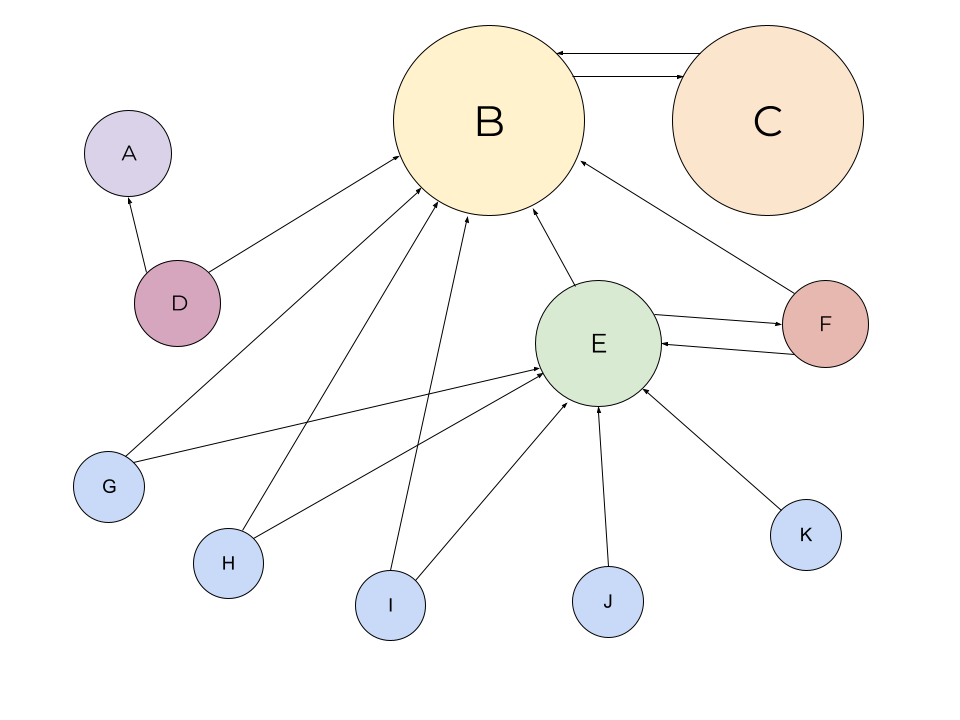
\includegraphics[width=\textwidth]{Wikipedia_Medium-graph.png}

We will run both PageRank and HITS on the network above.

\subsection{PageRank}

We expect vertices B and C to have the highest PageRank scores
because virtually every vertices points to it, either directly or through other vertices such as E.
We also expect E to have a fairly high PageRank score because there are many nodes pointing to it;
hoever, E points to B but B does not point to E, so E should have a lower PageRank than B.
Furthermore, we expect the vertices G, H, I, J, and K to have the lowest PageRank scores because
no vertices point towards them, and they only have edges pointing outwards.
Their PageRank scores should also be roughly equal since they each have a similar outgoing edge structure,
only pointing to 1 or 2 other vertices.

We run the following commands to apply PageRank on the graph.

\begin{minted}{julia}
$ julia
julia> using ScottyRank
julia> G=read_graph("data/medium-el.txt", filetype="el") # the graph is stored as an edge list
julia> pg = pagerank(G) # run PageRank on the graph
julia> pagerank_print(G, pg, num_lines=11)
\end{minted}

The printed result for \mintinline{julia}{pagerank_print} is shown below:

\begin{table}[h]
\begin{tabular}{lllll}
PageRank Score & Index & Vertex & In & Out\\
    0.3643 &        2 &         B& 7 &         1 \\
    0.3638 &         3 &         C& 1 &         1 \\
    0.0813 &         5 &         E& 6 &         3 \\
    0.0395 &         4 &         D& 1 &         2 \\
    0.0395 &         6 &         F& 1 &         2 \\
    0.0304 &         1 &         A& 1 &         0 \\
    0.0163 &         9 &         I& 0 &         2 \\
    0.0163 &        10 &         J& 0 &         1 \\
    0.0163 &        11 &         K& 0 &         1 \\
    0.0163 &         7 &         G& 0 &         2 \\
    0.0163 &         8 &         H& 0 &          2\\
\end{tabular}
\end{table}

The first column lists the calculated PageRank score and
the second lists the index of the vertex with that score.
The third, titled ``Vertex", is the letter assigned to that vertex (A for index 1, B for index 2, etc.).
The ``In" column displays the number of inbound edges to the corresponding vertex.
Similarly, the ``Out" columns displays the number of outbound edges from the corresponding vertex.

We see that, as expected, vertices B and C have the highest PageRank scores by far,
and E has the highest score of the remaining vertices.
Additionally, we see the vertices G, H, I, and J share the same lowest PageRank score of 0.0163.

\subsection{HITS on Medium-Sized Graph}

When predicting the results for HITS on the graph, we must recall the concepts behind HITS, namely
that a vertex pointing to vertices with high authority scores will have a high hub score,
and that a vertex which has vertices with high hub scores pointing to it will have a high authority score.

With this in mind, we see that vertices B and E should have the highest authority scores
simply because they have the greatest amount of vertices pointing towards them.

However, since B does not point towards many other authorities, its hub score should be low.
But E points to B, which is a high authority score vertex, so we should expect 
the hub score of E to be above average.

Similarly, the hub score of C should be relatively high since it points to B, but the authority score of C should be low because B does not have a high hub score.

Finally, we should expect the authority scores of G, H, I, J, and K all to be very low
because no vertices point towards them,
but their hub scores to be relatively high because they point to
one or both of the highest authority nodes-- B and E.

We run the following commands to apply HITS on the graph.

\begin{minted}{julia}
$ julia
julia> using ScottyRank
julia> G=read_graph("data/medium-el.txt", filetype="el") # the graph is stored as an edge list
julia> a,h = hits(G) # run HITS on the graph
julia> hits_print(G, a, h, num_lines=11)
\end{minted}

The printed result for \mintinline{julia}{hits_print} is shown below:

\begin{table}[h]
\begin{tabular}{lllll}
Authority Score & Index & Vertex & In & Out\\
    0.7554 &         2 &         B& 7 &         1 \\
    0.6388 &         5 &         E & 6 &         3 \\
    0.0870 &         4 &         D & 1 &         2 \\
    0.0870 &         6 &         F & 1 &         2 \\
    0.0779 &         1 &         A & 1 &         0 \\
    0.0000 &         3 &         C & 1 &         1 \\
    0.0000 &         7 &         G & 0 &         2 \\
    0.0000 &         8 &         H & 0 &         2 \\
    0.0000 &         9 &         I & 0 &         2 \\
    0.0000 &        10 &        J & 0 &         1 \\
    0.0000 &        11 &        K & 0 &         1 \\
\end{tabular}
\end{table}

\begin{table}[h]
\begin{tabular}{lllll}
Hub Score & Index & Vertex & In & Out\\
    0.4259 &         6 &        F & 1 &         2 \\
    0.4259 &         7 &        G & 0 &         2 \\
    0.4259 &         8 &        H & 0 &         2 \\
    0.4259 &         9 &        I & 0 &         2 \\
    0.2835 &         5 &        E & 6 &         3 \\
    0.2543 &         4 &        D & 1 &         2 \\
    0.2306 &         3 &        C & 1 &         1 \\
    0.1953 &        10 &       J & 0 &         1 \\
    0.1953 &        11 &       K & 0 &         1 \\
    0.0000 &         2 &        B & 7 &         1 \\
    0.0000 &         1 &        A & 1 &         0 \\
\end{tabular}
\end{table}

Like PageRank, the first column lists the calculated
authority score for the first table and the hub score for the second table.
The second column lists the index of the vertex with that score.
The third, titled ``Vertex", is the letter assigned to that vertex (A for index 1, B for index 2, etc.).
The ``In" column displays the number of inbound edges to the corresponding vertex.
Similarly, the ``Out" columns displays the number of outbound edges from the corresponding vertex.

As predicted, the authority scores of B and E are the highest, with C having a low authority score.
The vertices G, H, I, J, and K have authority scores of 0 because no vertices point to them.

Additionally, we see that the hub scores were also calculated as predicted--
the hub score of F was the highest because F pointed towards both B and E,
the two vertices with the highest authority scores. As justified in our predictions, G, H, I
have very high hub scores. However, J and K had lower hub scores because they only pointed to one of the main authorities.

\section{Code Appendix}

ADD AT END

\end{document}
